\section{Appendix}\label{sec:appendix}

\begin{figure}[h]
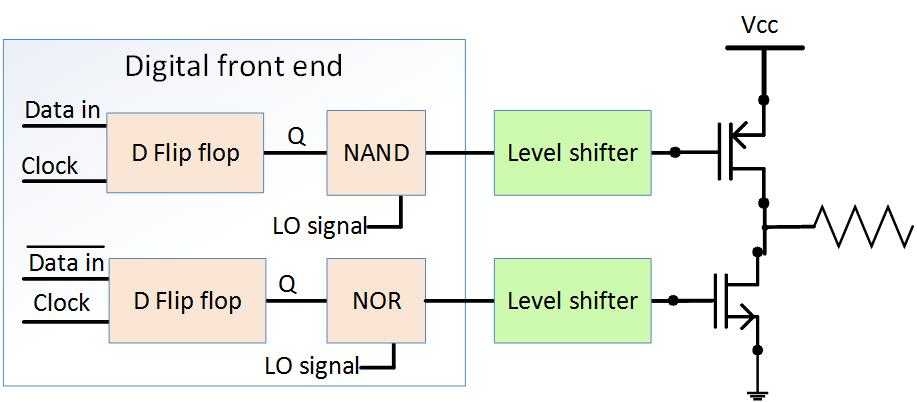
\includegraphics[width=0.5\textwidth]{Global_schematic_previous_group.jpg}
\caption{Global schematic of the previous group.}
\label{fig:Global_schematic_previous_group_figure}
\end{figure}

\begin{figure}[h]
 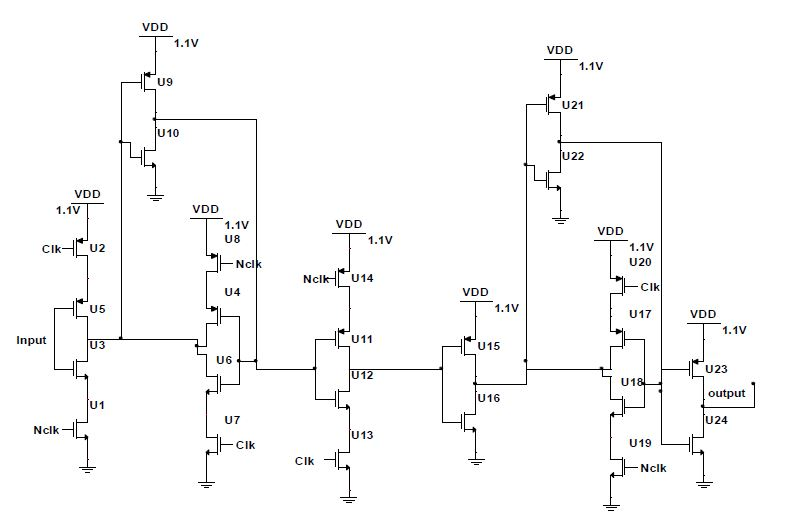
\includegraphics[width=0.5\textwidth]{D_flip_flop_schematic.jpg}
 \caption{ D flip flop schematic from previous group}
 \label{fig:D_flip_flop_ previous_group_figure}
\end{figure}

\begin{figure}[h]
 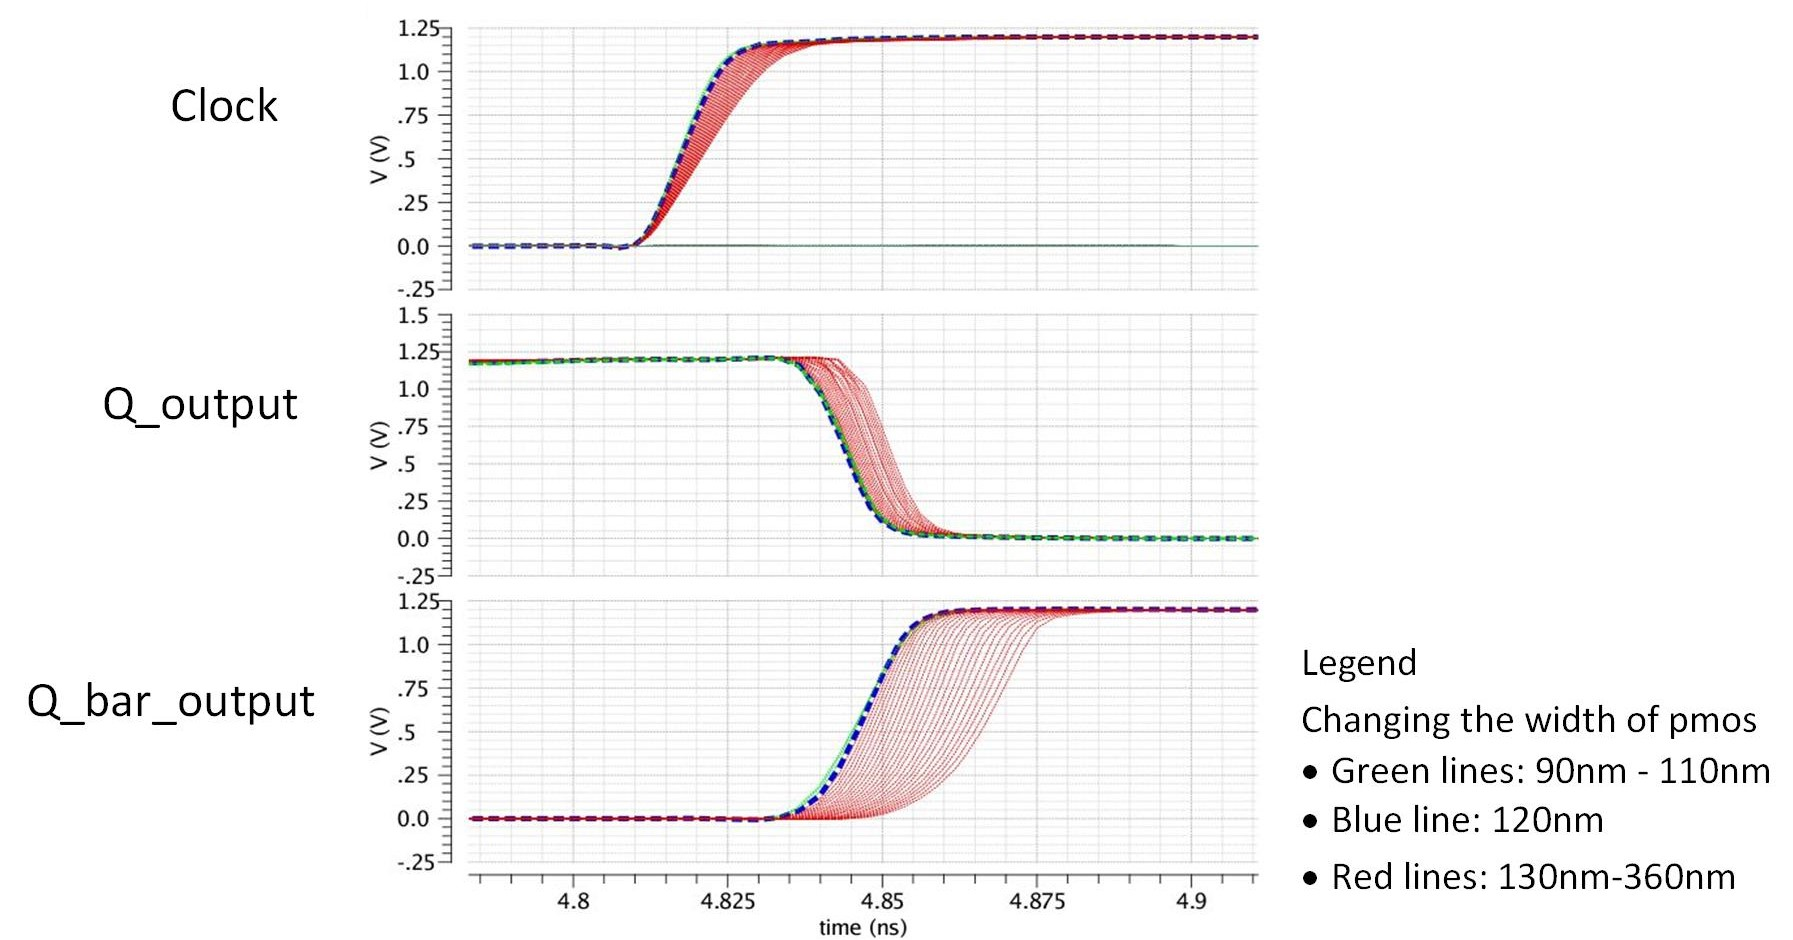
\includegraphics[width=0.5\textwidth]{Parameter_sweep_changing_w_high_to_low.jpg}
 \caption{Parametersweep of changing the width of the pmos when the data is low.}
 \label{fig:parametersweep_changing_w_high_to_low_figure}
\end{figure}

\begin{figure}[h]
 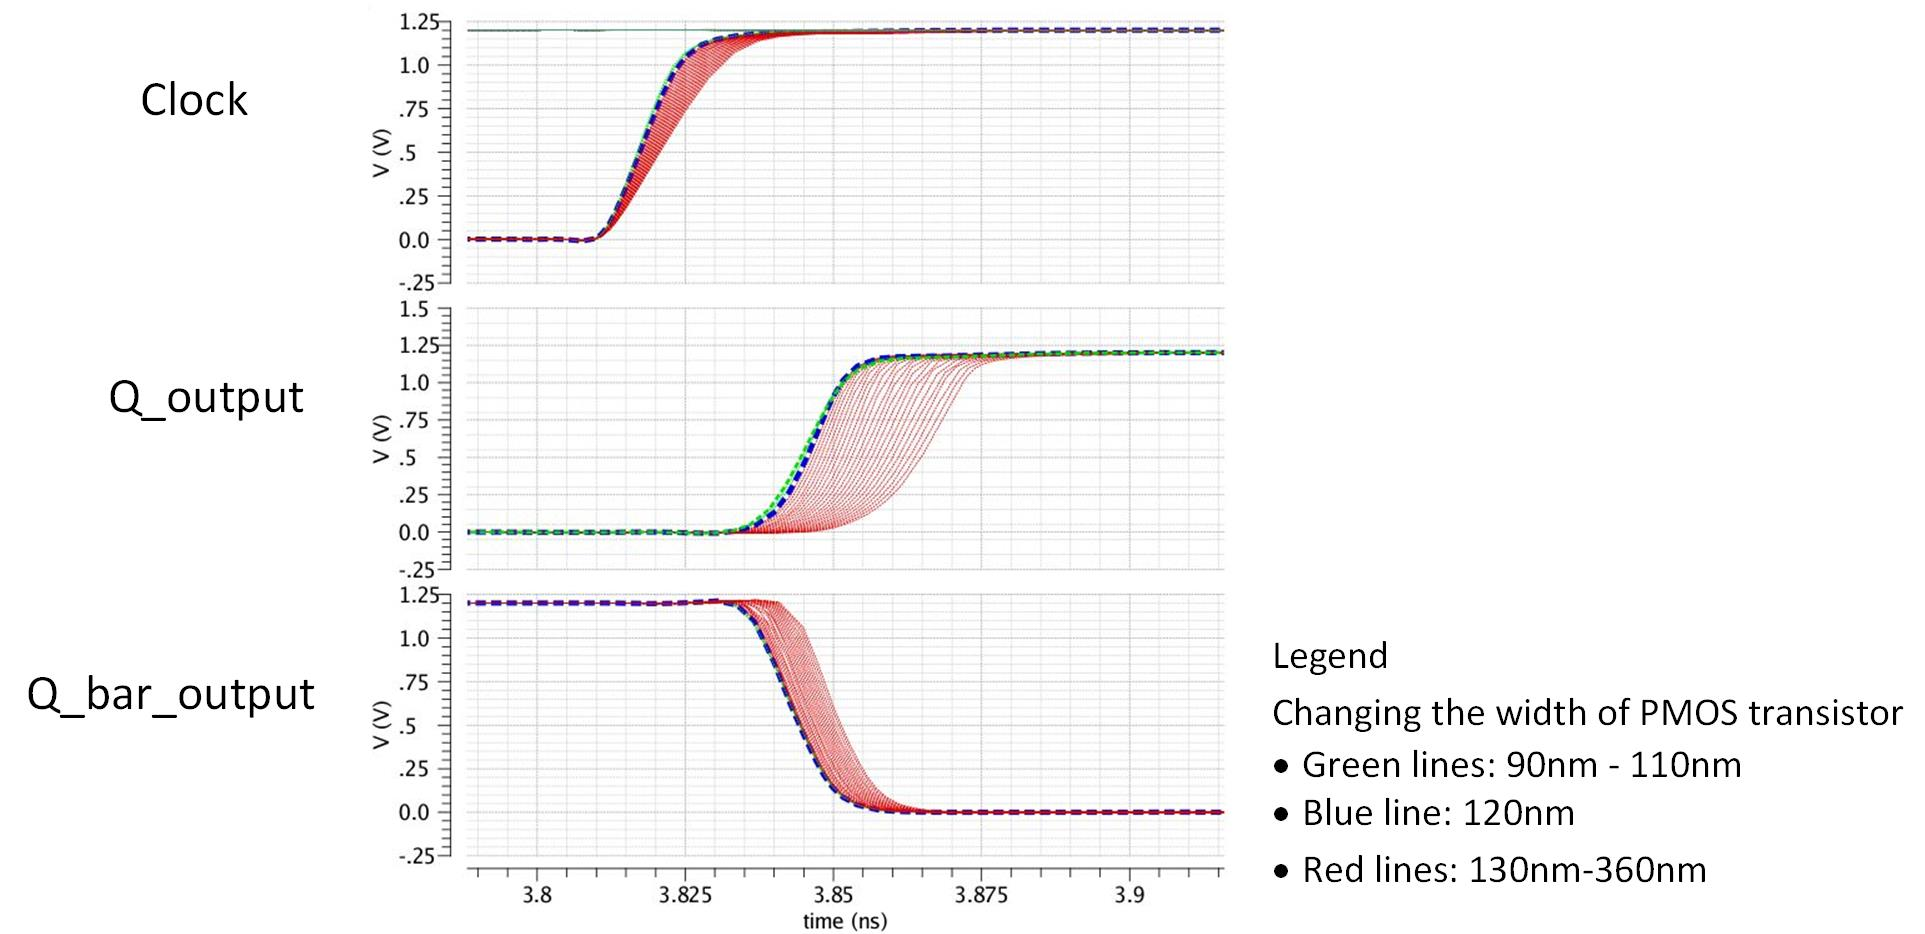
\includegraphics[width=0.5\textwidth]{Parameter_sweep_changing_w_low_to_high.jpg}
 \caption{Parametersweep of changing the width of the pmos when the data is high.}
 \label{fig:parametersweep_changing_w_low_to_high_figure}
\end{figure}

\begin{figure}[h]
 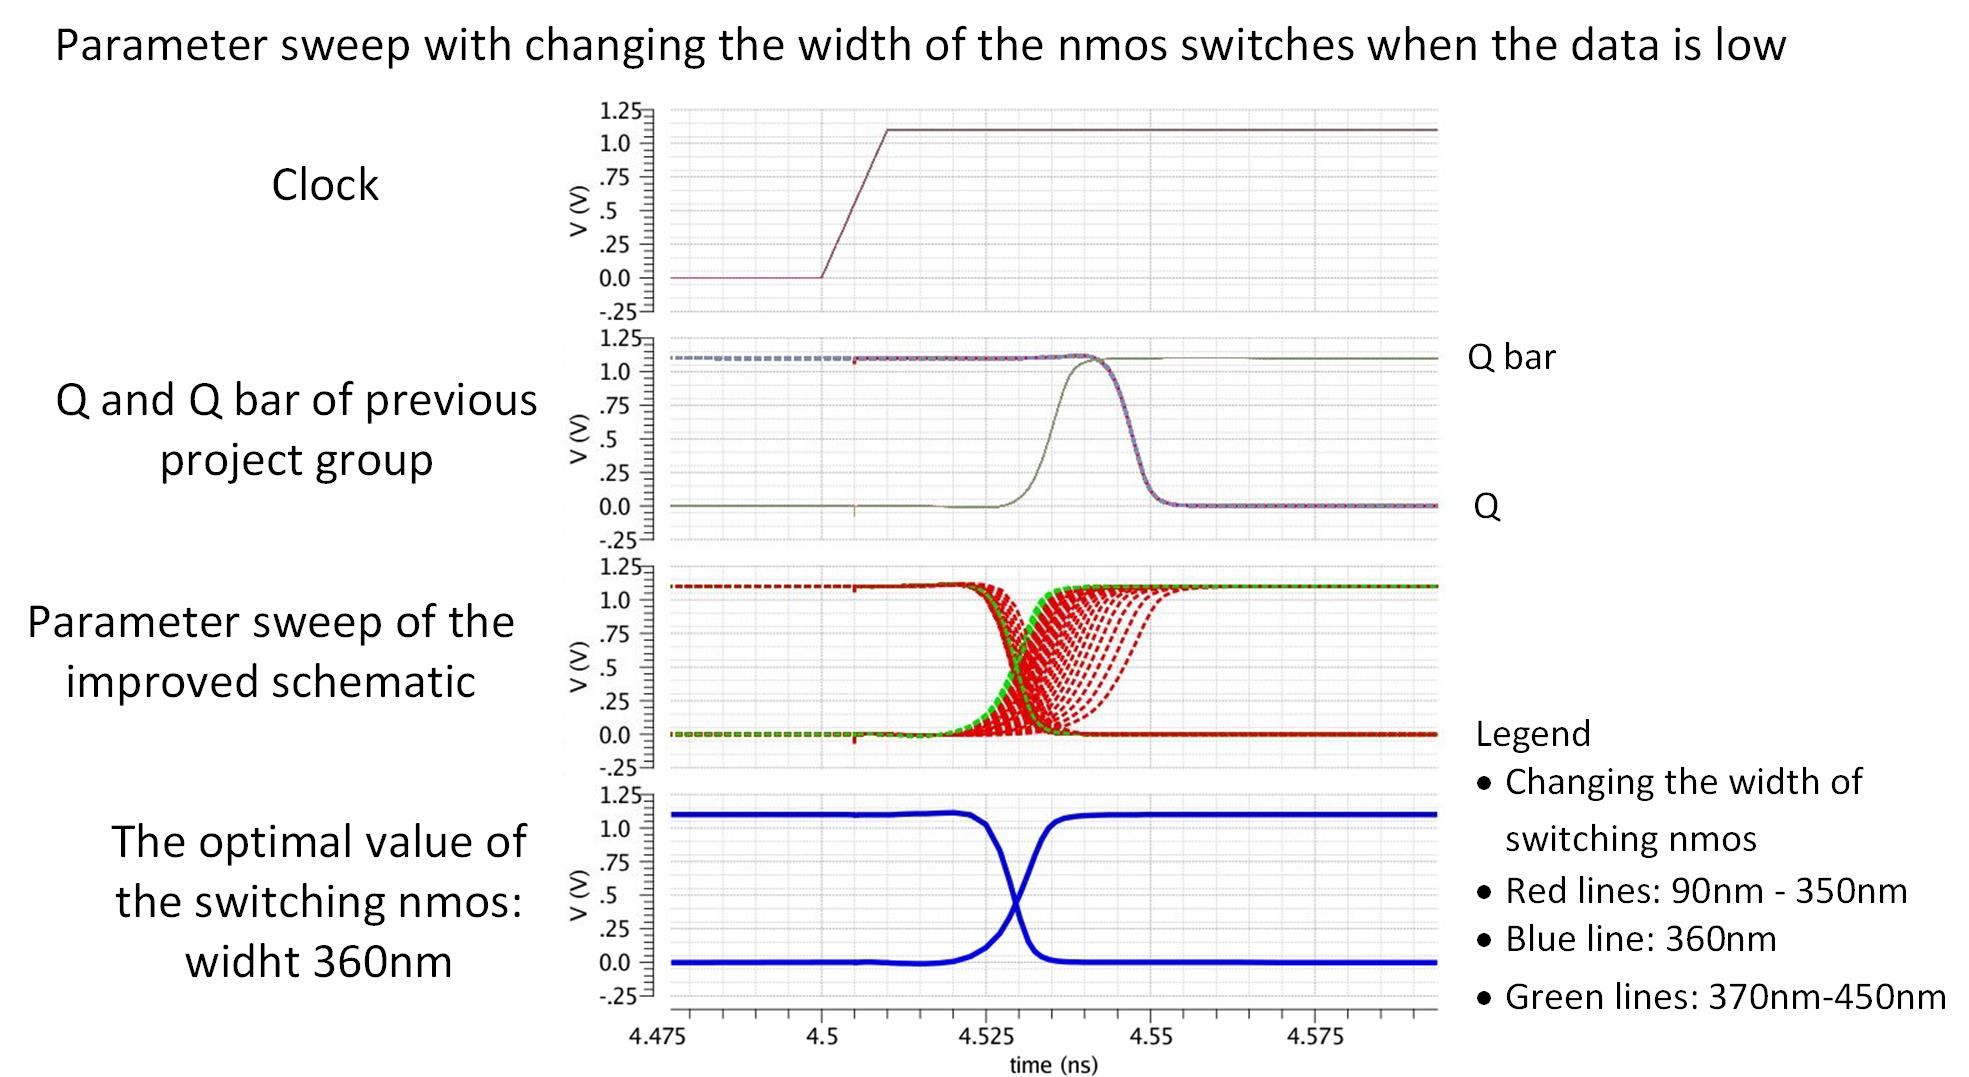
\includegraphics[width=0.5\textwidth]{Parameter_sweep_changing_w_of_the_swiching_nmos_high_to_low.jpg}
 \caption{Parameter sweep of changing the width of the switching nmos when the data is low.}
 \label{fig:Parameter_sweep_changing_w_of_the_swiching_nmos_high_to_low_figure}
\end{figure}

\begin{figure}[h]
 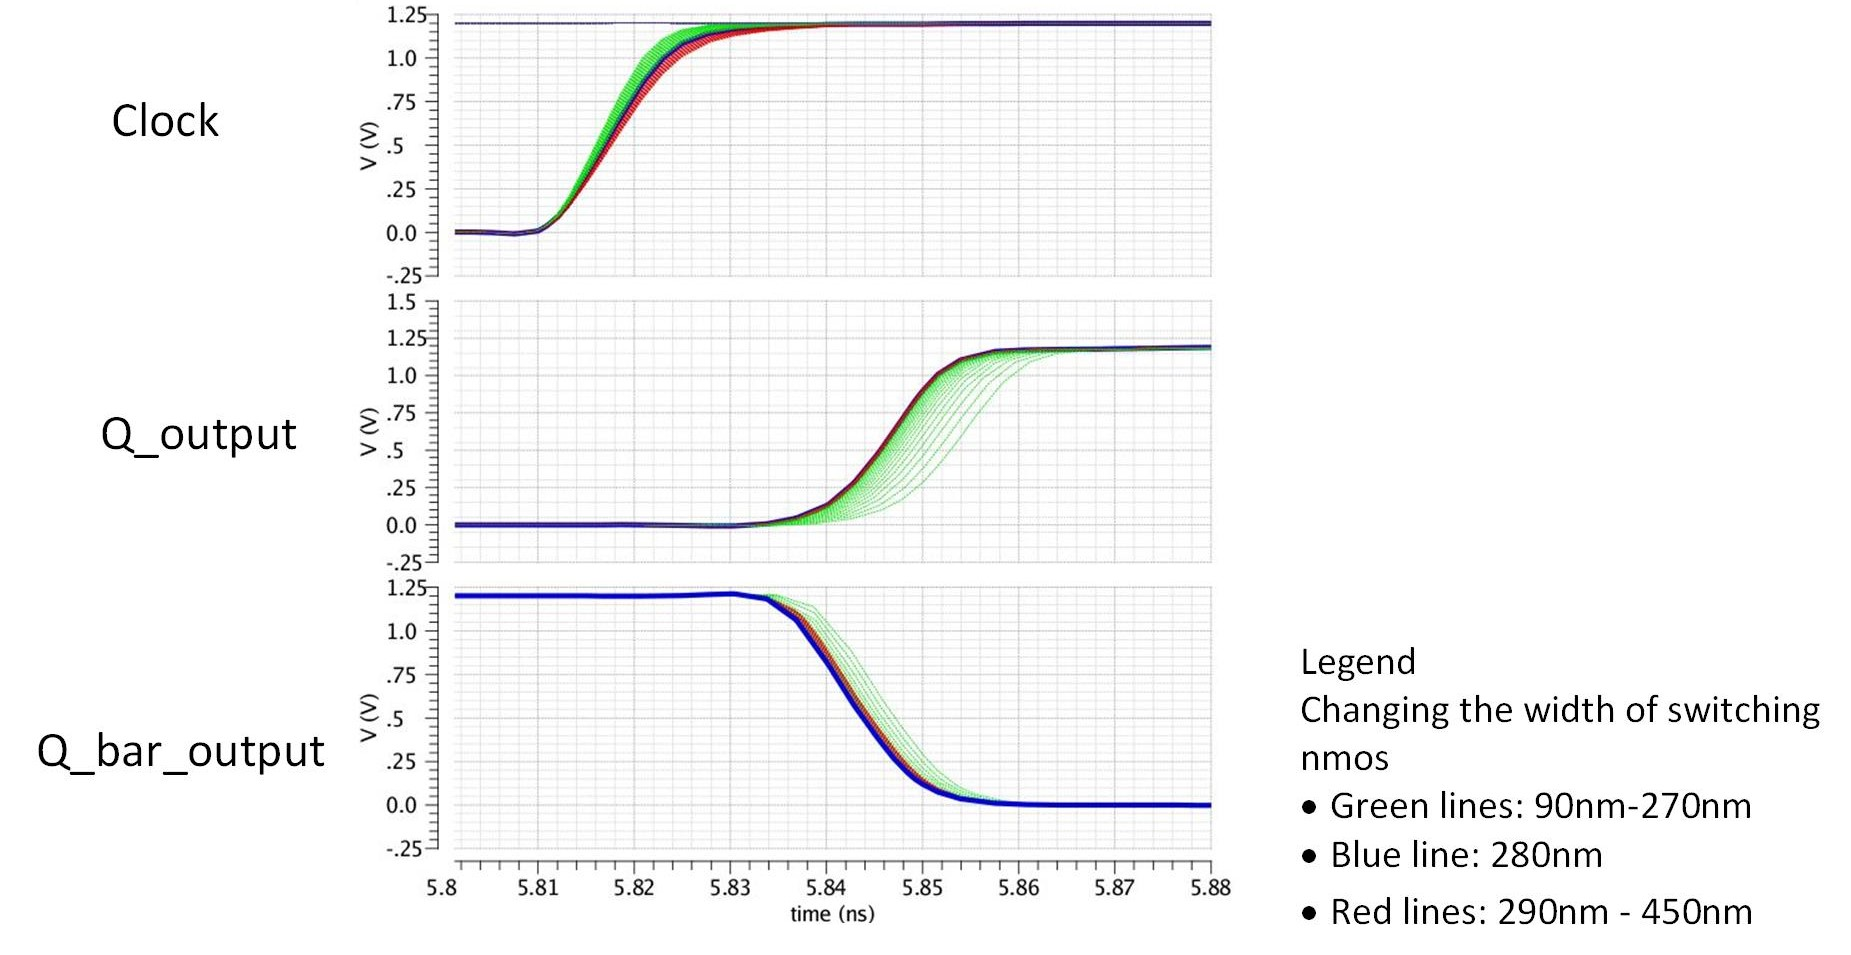
\includegraphics[width=0.5\textwidth]{Parameter_sweep_changing_w_of_the_swiching_nmos_low_to_high.jpg}
 \caption{Parameter sweep of changing the width of the switching nmos when the data is high}
 \label{fig:Parameter_sweep_changing_w_of_the_swiching_nmos_low_to_high_figure}
\end{figure}